% !Mode:: "TeX:UTF-8"
% !TEX program  = xelatex
\documentclass[a4paper]{article}
\usepackage{amsmath}
\usepackage{amssymb}
\usepackage{ctex}
%\usepackage{braket}
\usepackage[european]{circuitikz}
\usepackage{multirow}
\usepackage{geometry}
\geometry{left=2.5cm,right=2.5cm,bottom=2.5cm,top=2.5cm}
\title{模电实验报告2:单级放大电路实验(EWB仿真)}
\author{xy\quad 学号\quad 匡亚明学院}
\date{2019年2月29日}
\begin{document}
\maketitle
\bibliographystyle{unsrt}
%--------main-body------------

\section{实验目的}
\begin{enumerate}
\item 学习使用EWB仿真软件。
\item 使用EWB仿真软件对单机放大电路进行仿真。
\end{enumerate}

\section{实验仪器}
EWB仿真软件。

\section{实验内容}
\begin{enumerate}
\item 按图(\ref{cd})在EWB软件中搭建好电路图。
\begin{figure}[!h]
\begin{center}
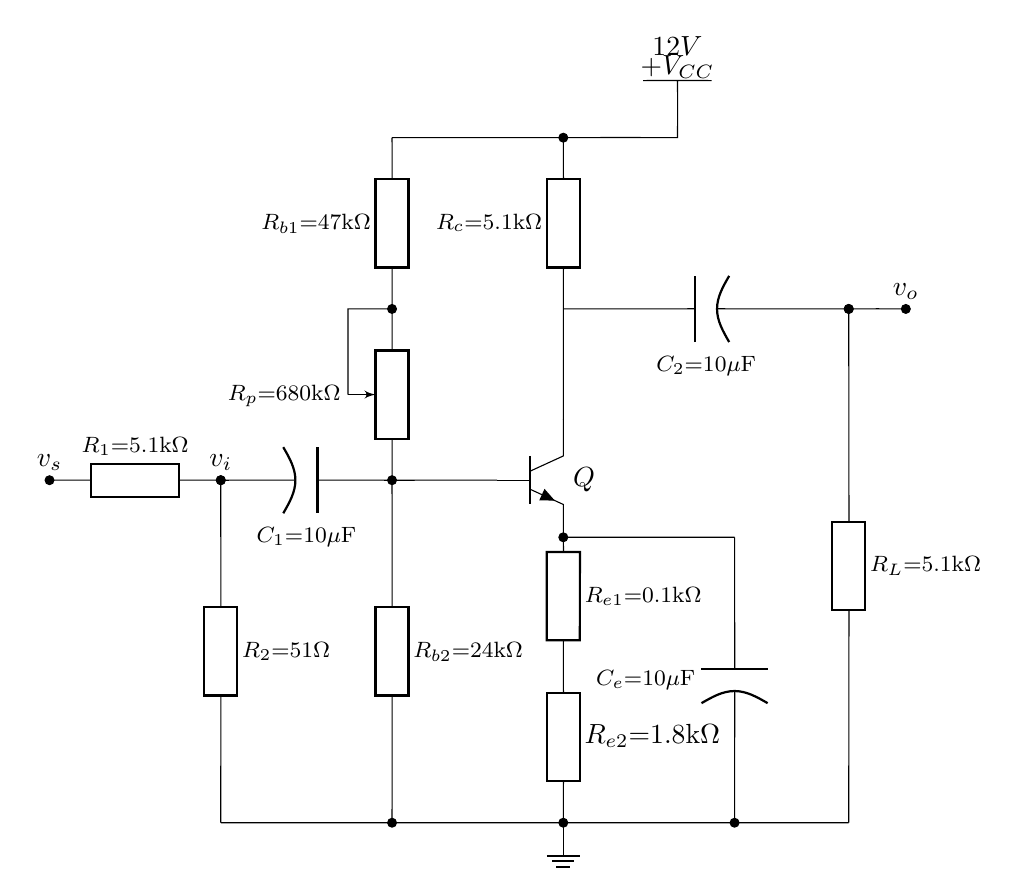
\begin{tikzpicture}[scale=1.45]
    \draw[color=black]
    (0,3) to [R, l =\footnotesize $R_1{=}5.1\text{k}\Omega$, *-*] (1.5,3)
    (1.5,3) to [R, l =\footnotesize $R_2{=}51\Omega$] (1.5,0)
    (1.5,3) to [pC, l_ =\footnotesize $C_1{=}10\mu\text{F}$, *-*] (3,3)
    (3,3) to [R, l =\footnotesize $R_{b2}{=}24\text{k}\Omega$] (3,0)
    (3,3) to [pR, l =\footnotesize $R_p{=}680\text{k}\Omega$, n = PR, -*] (3,4.5)
        to [R, l =\footnotesize $R_{b1}{=}47\text{k}\Omega$] (3,6)
    (3,4.5) -| (PR.wiper)
    (4.5,3) node[npn](NPN){}
    (3,3) to [-] (NPN.B)
    (NPN.E) to [R, l =\footnotesize $R_{e1}{=}0.1\text{k}\Omega$] (4.5, 1.5) to [R, l = $R_{e2}{=}1.8\text{k}\Omega$] (4.5,0)
    (NPN.C) to [-] (4.5,4.5) to [R, l =\footnotesize $R_c{=}5.1\text{k}\Omega$] (4.5,6) to [-] (3,6)
    (4.5,6) to [short, *-] (5.5,6)
    to [short] (5.5,6.5) to [short] (5.2,6.5) to [short] (5.8,6.5) to [short] (5.5,6.5)
    (5.5, 6.8) node{$12V$}
    (5.5, 6.62) node{$+V_{CC}$}
    (7,4.5) to [pC, *-, l =\footnotesize $C_2{=}10\mu\text{F}$] (4.5,4.5)
    (7,4.5) to [short, *-*] (7.5,4.5)
    (7,4.5) to [R, l =\footnotesize $R_L{=}5.1\text{k}\Omega$] (7,0)
    (4.5,2.5) to [short, *-] (6,2.5)
    (6,0) to [pC, l =\footnotesize $C_e{=}10\mu\text{F}$] (6,2.5)
    (1.5,0) to [short, -*] (3,0) to [short, -*] (4.5,0) to [short, -*] (6,0) to [-] (7,0)
    (4.5,0) node[ground](GND){}
	
    {[anchor = south] (0,3) node{$v_s$}}
    {[anchor = south] (1.5,3) node{$v_i$}}
    {[anchor = south] (7.5,4.5) node{$v_o$}}
    {[anchor = west] (4.5,3) node{$Q$}}
;
\end{tikzpicture}
\end{center}
\caption{共射放大电路}\label{cd}
\end{figure}
\item 调整静态\\
取仿真电路集电极静态电压为6V。万用表选择直流电压挡,开启EWB主窗口右上角的开关,调整基极偏置电位器$R_P$,发现680k$\Omega$过大,改用22k$\Omega$电位器,直至$V_c \approx$6V为止。
\item 测量交流放大倍数\\
双击示波器,出现示波器窗口。开启EWB主窗口右上角的开关。调整示波器A、B通道的位置,使两个通道的波形在示波器屏幕上分开,以利于观察。调整示波器的X轴时间刻度、Y轴电压刻度。按下EWB主窗口右上角的“Pause”键(暂停键),移动示波器屏幕下方的滚动条,将波形移入示波器的屏幕。再移动游标。
\item 测量放大器的幅频响应特性\\
双击波特仪,打开波特仪显示窗口。去掉负载,点击开始模拟,一段时间后暂停。记录波特仪的幅频响应曲线。记录峰值和峰值-3dB对应的频率。
\item 测量放大器的输入输出电阻\\
按书中要求调整相应电阻,进行模拟。
\end{enumerate}

\section{实验数据}
\begin{enumerate}
\item 调整静态\\
$R_P = 21.6\text{k}\Omega$,即$R_b = 72.6\text{k}\Omega$。
\begin{table}[!h]
\centering
\caption{调整静态}
\label{Q}
\begin{tabular}{c|c|c|c|c|c|c}
\hline
\multicolumn{4}{c|}{测量值}               & \multicolumn{3}{c}{测量计算值}      \\ \hline
$V_c$ & $R_P$         & $V_b$  & $V_e$  & $I_b$       & $I_c$   & $\beta$ \\ \hline
5.99V & 21.6k$\Omega$ & 2.881V & 2.249V & 5.564$\mu$A & 1.178mA & 211.796 \\ \hline
\end{tabular}
\end{table}
\item 交流放大倍数\\
\textbf{理论值计算:}\\
根据教材$^{\cite{jiaocai}}$的式(5.3.7b):
\begin{equation}
r_{be} = r_{bb'} + (1+\beta)\frac{26mV}{I_{EQ}}\label{rbe}
\end{equation}
及例(5.3.2)中的:
\begin{equation}
I_{EQ} \approx \beta I_{BQ}=211.796\times5.564 =1178.43 \mu\text{A}
\end{equation}
结合实际情况,取$r_{bb'} = 800\Omega$,可得:
\begin{equation}
r_{be} = 800\Omega + (1+211.796)\cfrac{26\text{mV}}{1178.43 \mu\text{A}} = 5.495\text{k}\Omega
\end{equation}
再根据式(5.3.8)并进行适当修正,有(下文计算中略去负号):
\begin{equation}
A_v = \cfrac{v_o}{v_i} = -\cfrac{\beta(R_L||R_c)}{R_b||r_{be}}\label{Av}
\end{equation}
\begin{enumerate}
\item 空载\\
空载即$R_L = 0$,将各数据代入式(\ref{Av})即得理论放大倍数:
\begin{equation}
A_v = -\cfrac{211.796\times5.1\text{k}\Omega}{72.6\text{k}\Omega || 5.495\text{k}\Omega} \approx 211.45
\end{equation}
将理论值与实验测量值填入表(\ref{Av_NL}):
\begin{table}[!h]
\centering
\caption{测量交流放大电路(空载)}
\label{Av_NL}
\begin{tabular}{c|c|c|c}
\hline
\multicolumn{2}{c|}{测量值} & 由测量值计算 & 理论估算值 \\ \hline
$v_i(mV)$   & $v_o(V)$  & $A_V$  & $A_V$ \\ \hline
2.932                 & 0.632         & 215.64    & 211.45      \\ \hline
5.864                 & 1.257         & 214.36    & 211.45      \\ \hline
8.797                 & 1.865         & 212.00    & 211.45      \\ \hline
\end{tabular}
\end{table}

误差为:
\begin{eqnarray}
Error(v_i=3mV) &=& \frac{215.64-211.45}{211.45}\times 100\% = -1.98\%\\
Error(v_i=6mV) &=& \frac{214.36-211.45}{211.45}\times 100\% = -1.38\%\\
Error(v_i=9mV) &=& \frac{212.00-211.45}{211.45}\times 100\% = -0.26\%
\end{eqnarray}
\item 有载\\
有载即$R_L = 5.1\text{k}\Omega$和$R_L = 2.2\text{k}\Omega$,将各数据代入式(\ref{Av})即得理论放大倍数:
\begin{eqnarray}
A_v(R_L = 5.1\text{k}\Omega) &=& -\cfrac{211.796\times(5.1\text{k}\Omega || 5.1\text{k}\Omega)}{72.6\text{k}\Omega || 5.495\text{k}\Omega} \approx 105.69\\
A_v(R_L = 2.2\text{k}\Omega) &=& -\cfrac{211.796\times(5.1\text{k}\Omega || 2.2\text{k}\Omega)}{72.6\text{k}\Omega || 5.495\text{k}\Omega} \approx 63.70
\end{eqnarray}
\begin{table}[!h]
\centering
\caption{测量交流放大倍数(有载)}
\label{Av_L}
\begin{tabular}{c|c|c|c|c}
\hline
负载           & \multicolumn{2}{c|}{测量值}                 & 由测量值计算 & 理论估算值 \\ \hline
$R_L$        & $v_i(mV)$ & $v_o(mV)$ & $A_V$  & $A_V$ \\ \hline
5.1$k\Omega$ & 2.931 & 324.78        & 110.81 & 105.69      \\ \hline
2.2$k\Omega$ & 2.931 & 197.909       & 67.52  & 63.70    \\ \hline
\end{tabular}
\end{table}

误差为:
\begin{eqnarray}
Error(R_L = 5.1\text{k}\Omega) &=& \frac{110.81-105.69}{105.69}\times 100\% = 4.84\%\\
Error(R_L = 2.2\text{k}\Omega) &=& \frac{67.52-63.70}{63.70}\times 100\% = 6.00\%
\end{eqnarray}
\end{enumerate}
\item 幅频响应特性\\
取中频为10kHz,测得对应的通频带为:\\
$f_L$ = 701.704Hz,$f_H$ = 7.764MHz。\\
如图(\ref{bode})
\begin{figure}[!h]
\centering
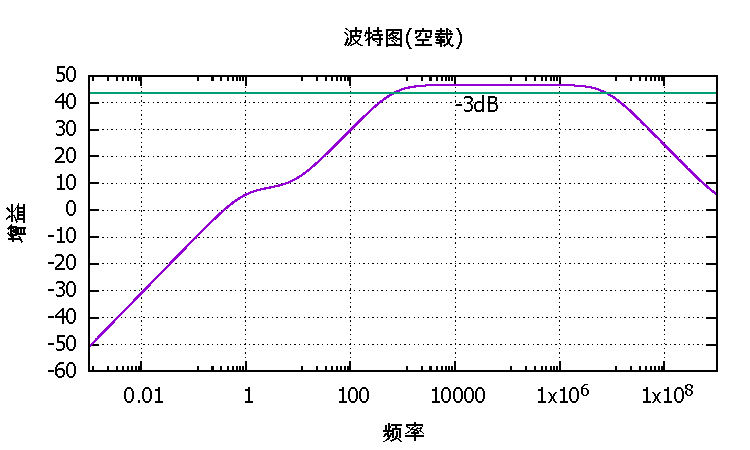
\includegraphics[width=12cm]{fig/BodeNL.pdf}\\
\caption{波特图(空载)}\label{bode}
\end{figure}
\item 输入输出电阻\\
\textbf{理论值计算:}\\
根据教材(5.3.9)和(5.3.10)两式,可以得出输入输出电阻的理论值:
\begin{eqnarray}
r_i &=& R_b || r_{be} = 72.6\text{k}\Omega || 5.495\text{k}\Omega = 5.11\text{k}\Omega\\
r_o &\approx& R_c = 5.1\text{k}\Omega
\end{eqnarray}
测得的相关数据为:
\begin{enumerate}
\item 输入\\
$V_s = 36\text{mV}$\\
$V_i = 16.121\text{mV}$\\
$r_i = \cfrac{R_s}{\frac{V_s}{V_i}-1} = 5.59\text{k}\Omega$
\item 输出\\
$V_o(\text{空载}) = 632.249\text{mV}$\\
$V_o(\text{有载}) = 324.783\text{mV}$\\
$r_o = \left(\cfrac{V_{o}(\text{空载})}{V_{o}(\text{有载})}-1\right)R_L = 4.83\text{k}\Omega$
\end{enumerate}
\begin{table}[!h]
\centering
\caption{测量输入输出电阻}
\label{table8}
\begin{tabular}{c|c|c|c|c|c|c|c}
\hline
\multicolumn{4}{c|}{测输入电阻$r_i$ $R_s = 5.1k\Omega$} & \multicolumn{4}{c}{测输出电阻$r_o$}                             \\ \hline
\multicolumn{2}{c|}{测量值}     & 测量计算值    & 理论估算值    & \multicolumn{2}{c|}{测量值}                    & 测量计算值 & 理论估算值 \\ \hline
$V_s(mV)$     & $V_i(mV)$    & $r_i$    & $r_i$    & $V_o, R_L\to\infty$ & $V_o, R_L=5.1k\Omega$ & $r-o$ & $r_o$ \\ \hline
36  &  16.121   & 5.59 k$\Omega$ & 5.11\text{k}$\Omega$ & 632.249$\text{mV}$  & 324.783$\text{mV}$  & 4.83k$\Omega$  & 5.1\text{k}$\Omega$ \\ \hline
\end{tabular}
\end{table}
则输入输出电阻的误差为:
\begin{eqnarray}
Error(r_i) &=& \cfrac{5.59\text{k}\Omega - 5.11\text{k}\Omega}{5.11\text{k}\Omega}\times 100\% = 9.39\%\\
Error(r_o) &=& \cfrac{4.83\text{k}\Omega - 5.1\text{k}\Omega}{5.1\text{k}\Omega}\times 100\% = -5.29\%
\end{eqnarray}
\end{enumerate}	

\section{思考题}
\subsection{将$C_e$改为100$\mu$F,进行仿真。}

%--------bib------------------
\bibliography{ref}
\end{document}